\documentclass[letterpaper, 11pt, oneside]{book}

\usepackage{style}  % If you feel like procrastinating, mess with this file
\usepackage{algo}   % Thank you Jeff, very cool!

\addbibresource{refs.bib}

% Required reading
% https://jmlr.csail.mit.edu/reviewing-papers/knuth_mathematical_writing.pdf
%   Along with required viewing:
%   https://www.youtube.com/watch?v=N6QEgbPWUrg&list=PLOdeqCXq1tXihn5KmyB2YTOqgxaUkcNYG
% https://faculty.math.illinois.edu/~west/grammar.html

% % % % % % % % % %
%     Cursor      %
%     Parking     %
%     Lot         %
% % % % % % % % % %

% Disable check for mismatched parens/brackets/braces
%   chktex-file 9
% Disable check for different counts of parents/brackets/braces
%   chktex-file 17
% Exclude these environments from syntax checking
%   VerbEnvir { tikzcd }

\regtotcounter{figure}

\title{\vspace{-100pt} 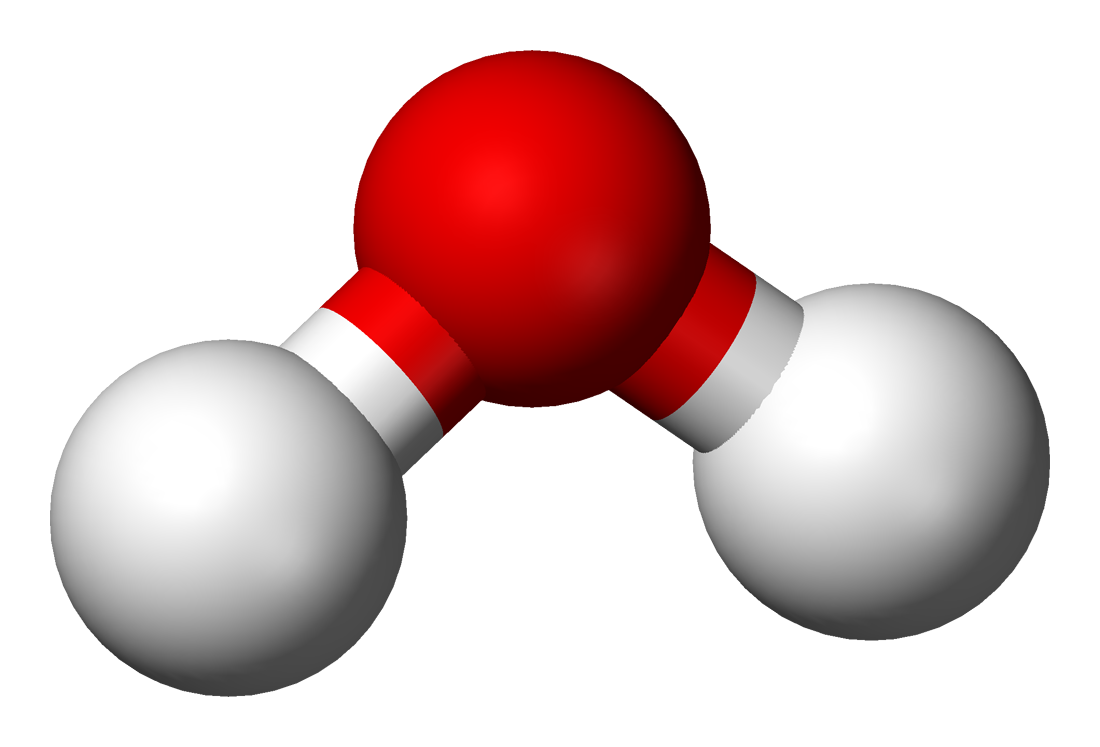
\includegraphics[width=0.75\textwidth]{figs/water.png} \\ {\Huge Representation Theory Notes and Exercises} \\ {\small With $\total{figure}$ Figures}}
\author{\Large Anakin Dey}
\DTMsavenow{now}
\date{\small Last Edited on \today\ at \DTMfetchhour{now}:\DTMfetchminute{now}}

% Cover page number chicanery
\newcommand{\CoverName}{Cover}

\begin{document}
\frontmatter
\renewcommand{\thepage}{\CoverName}
\maketitle

\pagenumbering{roman}

\section*{TODOs}

\quest{Change the style of enumerates from ``1.'' to ``(1)''}

\quest{Proper Exercise Header}

\quest{Proper Chapter Header}

\quest{Remove indent at end of thmtool environments}

\tableofcontents
\clearpage


\listoftheorems[ignoreall, show={defn}, title={List of Definitions}]

\listoftheorems[ignoreall, show={ex}, title={List of Examples and Counterexamples}]

\chapter*{Preface}

This is a set of notes on group representation theory mainly based on J.P. Serre's text \emph{Linear Representations of Finite Groups}~\cite{book:SerreLinReps}.
Occasionally, other sources may be used, such as the set of notes by Charles Rezk created for Math 427~\cite{note:rezk_reps}.
The goal of these notes is to eventually work towards algebraic combinatorics such as Fulton's text \emph{Young Tableaux}~\cite{book:FultonTableaux}, as much of algebraic combinatorics is motivated by questions stemming from representation theory.
At the time of writing this, another goal is the applications of representation theory to computational complexity: see~\cite{misc:PanovaComputational} for a recent survey on this connection.

\mainmatter

\chapter{Generalities on Linear Representations}

Unless otherwise specified, $V$ will denote a vector space, usually over the field $\C$.
We will restrict ourselves to finite dimensional vector spaces.
Similarly, we will restrict ourselves to finite groups.

\begin{defn}[Linear Representation, Representation Space]
  Let $G$ be a group with identity $e$.
  A \emph{linear representation} of $G$ in $V$ is a homomorphism $\rho\colon G \to \GL(V)$.
  We will frequently, and often interchangeably, write $\rho_{s} \defeq \rho(s)$.
  Given $\rho$, we will say that $V$ is a \emph{representation space} or \emph{representation} of $G$.
\end{defn}

\begin{defn}[Degree]
  Let $\rho\colon G \to V$ be a representation of $G$ in a vector space $V$.
  Then the \emph{degree} of $\rho$ is $\dim(V)$.
\end{defn}

Let $\rho\colon G \to V$ be a representation of $G$ in a vector space $V$ with $n \defeq \dim(V)$.
Fix a basis $(e_{j})$ of $V$.
Then since each $\rho_{s}$ is an invertible linear transformation of $V$, we may define an $n \times n$ matrix $R_{s} \equiv (r_{ij}(s))$ where each $r_{ij}(s)$ is defined by the identity
\[
  \rho_{s}(e_{j}) = \sum_{i = 1}^{n} r_{ij}(s) e_{i}.
\]

\begin{defn}[Matrix of a Representation]
  We call $R_{s} = (r_{ij}(s))$ above the \emph{matrix of $\rho_{s}$} with respect to the basis $(e_{j})$.
\end{defn}
Note that $R_{s}$ satisfies the following:
\begin{align*}
  \det(R_{s}) \neq 0, && R_{st} = R_{s} \cdot R_{t} \equiv r_{ij}(st) = \sum_{k = 1}^{n} r_{ik}(s) \cdot r_{kj}(s) \quad \forall s, t \in G.
\end{align*}

\clearpage

Recall that two $n \times n$ matrices $A, A'$ are \emph{similar} if there exists an invertible matrix $T$ such that $T A = A' T$.
We may extend this notion to representations.
\begin{defn}[Similar/Isomorphic Representations]
  Let $\rho$ and $\rho'$ be two representations of the same group $G$ in vector spaces $V$ and $V'$ respectively.
  We say $\rho$ and $\rho'$ are \emph{similar} or \emph{isomorphic} if there exists an isomorphism $\tau \colon V \to V'$ such that for all $s \in G$, $\tau$ satisfies $\tau \circ \rho(s) = \rho'(s) \circ \tau$.
  If $R_{s}, R'_{s}$ are the corresponding matrices then this is equivalent to saying there exists an invertible matrix $T$ such that $T R_{s} = R'_{s} T$ for all $s \in G$.
\end{defn}
Note that if $\rho$ and $\rho'$ are isomorphic, then they must have the same degree.

We now give some examples of these things.
\begin{ex}[Unit/Trivial Representation]\label{ex:unit_trivial_representation}
  Let $G$ be a finite group.
  Representations of degree $1$ must be of the form $\rho\colon G \to \C^{\times}$.
  Since elements $s$ of $G$ are of finite order, $\rho(s)$ must also be of finite order.
  Thus, for all $s \in G$, $\rho(s)$ is a root of unity.
  If we take $\rho(s) = 1$ for all $s \in G$, we obtain the \emph{unit} or \emph{trivial} representation of $G$.
  This also means that $R_{s} = 1$ for all $s$.
\end{ex}

\begin{ex}[Regular Representation]\label{ex:regular_representation_Z3}
  Let $g$ be the order of $G$, and let $V$ be a vector space of dimension $g$ with a basis $(e_{t})_{t \in G}$.
  For each $s \in G$, define $\rho_{s}$ as the linear map $\rho_{s}\colon V \to V$ such that $\rho_{s}(e_{t}) = e_{st}$.
  This is a linear representation of $G$ called the \emph{regular} representation of $G$.
  Since for each $s \in G$, $e_{s} = \rho_{s}(e_{1})$ and thus the images of $e_{1}$ form a basis of $V$.
  Conversely, let $W$ be a representation of $G$ with a vector $w$ satisfying the collection of all $\rho_{s}(w)$, $s \in G$, forms a basis of $W$.
  Then $W$ is isomorphic to the regular representation of $G$ by the isomorphism $\tau(e_{s}) = \rho_{s}(w)$.

  For example, let $G = \Z_{3}$ and $V = \C^{3}$ with $e_{0} = (1, 0, 0)$, $e_{1} = (0, 1, 0)$, and $e_{2} = (0, 0, 1)$.
  Then for example, $\rho_{0}, \rho_{1}, \rho_{2}\colon \C^{3} \to \C^{3}$ are the linear maps such that
  \begin{align*}
    \rho_{0}(e_{0}) = e_{0 + 0} = e_{0} && \rho_{0}(e_{1}) = e_{0 + 1} = e_{1} && \rho_{0}(e_{2}) = e_{0 + 2} = e_{2} \\
    \rho_{1}(e_{0}) = e_{1 + 0} = e_{1} && \rho_{1}(e_{1}) = e_{1 + 1} = e_{2} && \rho_{1}(e_{2}) = e_{1 + 2} = e_{0} \\
    \rho_{2}(e_{0}) = e_{2 + 0} = e_{2} && \rho_{2}(e_{1}) = e_{2 + 1} = e_{0} && \rho_{2}(e_{2}) = e_{2 + 2} = e_{1}
  \end{align*}
  With this, the matrix representations of $\rho_{0}, \rho_{1}$ and $\rho_{2}$ is similarly straightforward:
  \begin{align*}
    R_{0} = \begin{pmatrix} 1 & 0 & 0 \\ 0 & 1 & 0 \\ 0 & 0 & 1 \end{pmatrix} && R_{1} = \begin{pmatrix} 0 & 0 & 1 \\ 1 & 0 & 0 \\ 0 & 1 & 0 \end{pmatrix} && R_{2} = \begin{pmatrix} 0 & 1 & 0 \\ 0 & 0 & 1 \\ 1 & 0 & 0 \end{pmatrix}
  \end{align*}
\end{ex}

\clearpage

\begin{ex}[Permutation Representation]\label{ex:perm_rep}
  We may generalize the regular representation to any group action $G \acts X$, $X$ a finite set.
  Recall that for such an action, the map $x \mapsto sx$ for each $s \in G$ is a permutation $X \tofrom X$.
  Let $V$ be a vector space with dimension the size of $X$, and so a basis $(e_{x})_{x \in X}$.
  Define a representation $\rho$ of $G$ by defining $\rho_{s}$ as the linear map sending $e_{x} \mapsto e_{sx}$.
  This representation is known as the \emph{Permutation} representation of $G$ associated with $X$.
  If we consider $X = [n]$ and $G = S_{n}$, then take $V = \C^{n}$ as our vector space and $e_{i}$ as the standard basis vector.
  Then $\rho_{\sigma}(e_{j}) = e_{\sigma_{j}}$.
  Thus for each $\sigma \in S_{n}$, we have that $R_{\sigma} = (r_{ij}(\sigma))$ where entry $r_{ij}(\sigma) = 1$ if $i = \sigma(j)$ and $0$ otherwise.
\end{ex}

\begin{defn}[Stable/Invariant Subspaces, Subrepresentation]
  Let $\rho\colon G \to \GL(V)$ be a linear representation and $W \subseteq V$ a subspace of $V$.
  We say that $W$ is \emph{stable} under the action of $G$ if $x \in W$ implies that $\rho_{s}(x) \in W$ for all $s \in G$.,
  Thus, the restriction $\rho_{s}^{W} \defeq \rho_{s}\mid_{W}$ is an isomorphism of $W$ onto itself.
  Restrictions satisfy the property that $\rho_{s}^{W} \circ \rho_{t}^{W} = \rho_{st}^{W}$.
  Thus, $\rho^{W}\colon G \to \GL(W)$ is a linear representation of $G$ in $W$ and we say that $W$ is a \emph{subrepresentation} of $V$.
\end{defn}

\begin{ex}[Subrepresentations of the Regular Representation]\label{ex:subrep_reg_rep}
  Let $G$ be a group.
  Recall the regular representation $V$ given in \Cref{ex:regular_representation_Z3}.
  Let $W$ be the 1 dimensional subspace of $V$ generated by the element $x = \sum_{s \in G} e_{s}$.
  Then note that $\rho_{s}(x) = x$ for all $s \in G$ and thus $W$ is a subrepresentation of $V$.
  Furthermore, this is isomorphic to the unit representation \Cref{ex:unit_trivial_representation} with $\tau\colon C^{\times} \to W$ such that $\tau(1) = x$.
  For example, let $G = \Z_{3}$ and $\rho\colon \Z_{3} \to \GL(\C^{3})$ the representation given in \Cref{ex:regular_representation_Z3}.
  Then $x = (1, 1, 1)$ and for example we have that
  \[
    \rho_{1}(x) = \rho_{1}(e_{0}) + \rho_{1}(e_{1}) + \rho_{1}(e_{2}) = e_{1} + e_{2} + e_{0} = x.
  \]
\end{ex}

\begin{thrm}\label{thrm:stable_complements_of_subspace}
  Let $\rho\colon G \to \GL(V)$ be a linear representation of $G$ in $V$ and let $W$ be a subspace of $V$ stable under $G$.
  Then there exists a complement $W^{0}$ of $W$ in $V$ which is stable under $G$.
\end{thrm}
\begin{pf}
  Let $W'$ be an arbitrary complement of $W$ in $V$, and let $p\colon V \to W$ be the projection.
  Then we form the average $p^{0}$ of conjugates of $p$ by elements in $G$:
  \[
    p^{0} \defeq \frac{1}{\abs{G}} \sum_{t \in G} \rho_{t} \circ p \circ \rho_{t}^{-1}.
  \]
  Since $p\colon V \to W$ and $\rho_{t}$ preserves $W$, we have that $p^{0}$ maps $V$ onto $W$.
  Furthermore, note that $\rho_{t}^{-1}$ also preserves $W$.
  \clearpage
  Thus we have that
  \begin{align*}
    (p \circ \rho_{t}^{-1})(x) = \rho_{t}^{-1}(x), && (\rho_{t} \circ p \circ \rho_{t}^{-1})(x) = x, && p^{0}(x) = x.
  \end{align*}
  Thus, $p^{0}$ is a projection of $V$ onto $W$, corresponding to some complement $W^{0}$ of $W$.
  Moreover, we have that $\rho_{s} \circ p^{0} = p^{0} \circ \rho_{s}$ for all $s \in G$ because
  \[
    \rho_{s} \circ p^{0} \circ \rho_{s}^{-1} = \frac{1}{\abs{G}} \sum_{t \in G} \rho_{s} \circ \rho_{t} \circ p \circ \rho_{t}^{-1} \circ \rho_{s}^{-1} = \frac{1}{\abs{G}} \sum_{t \in G} \rho_{st} \circ p \rho_{st}^{-1} = p^{0}.
  \]
  Now suppose that $x \in W^{0}$ and $s \in G$, we have that $p^{0}(x) = 0$ and hence $(p^{0} \circ \rho_{s})(x) = (\rho_{s} \circ p^{0})(x) = 0$, meaning that $\rho_{s}(x) \in W^{0}$.
  This, $W^{0}$ is stable under $G$.
\end{pf}

Suppose that $V$ had an inner product $\inner{x, y}$, and furthermore suppose this inner product was invariant under $G$ meaning that for all $s \in G$, $\inner{\rho_{s}(x), \rho_{s}(y)} = \inner{x, y}$.
We may also reduce to this case by replacing $\inner{x, y}$ with $\sum_{t \in G}\inner{\rho_{t}(x), \rho_{t}(y)}$.
With this, the orthogonal complement $W^{\bot}$ of $W$ in $V$ is a complement of $W$ stable under $G$.
Note that the invariance of $\inner{x, y}$ means that if $(e_{i})$ is an orthonormal basis of $V$, then $R_{s}$ is a unitary matrix.

Using the notation of \Cref{thrm:stable_complements_of_subspace}, let $x \in V$ and $w, w^{0}$ be the projections of $x$ on $W$ and $W^{0}$ respectively.
Thus for all $s \in G$, $\rho_{s}(x) = \rho_{s}(w) + \rho_{s}(w^{0})$.
Since $W$ and $W^{0}$ are stable under $G$, we have that $\rho_{s}(w) \in W$ and $\rho_{s}(w^{0}) \in W^{0}$.
This means that $\rho_{s}(w)$ and $\rho_{s}(w^{0})$ are the projections of $\rho_{s}(x)$ and in turn the representations of $W$ and $W^{0}$ determine the representations of $V$.
\begin{defn}[Direct Sum of Representations]
  Given the above, we write $V = W \oplus W^{0}$ as the \emph{direct sum} of $W$ and $W^{0}$.
  We identify elements $v \in V$ as pairs $(w, w^{0})$ given by their projections.
\end{defn}
If the representations $W$ and $W^{0}$ are given in matrices $R_{s}$ and $R_{s}^{0}$, then the matrix form of the representation $V$ is given by
\[
  \begin{pmatrix} R_{s} & 0 \\ 0 & R_{s}^{0} \end{pmatrix}.
\]
Similar results hold for arbitrarily many, but finite, direct sums of representations.

The above is a discussion on how to compose two or more representations into one larger representation.
The natural question is then about the opposite.
\begin{defn}[Irreducible/Simple Representations]
  Let $\rho\colon G \to \GL(V)$ be a linear representation of $G$.
  Then this representation is \emph{irreducible} or \emph{simple} if $V$ has no subspaces stable under $G$ besides $0$ and $V$ itself.
\end{defn}
By \Cref{thrm:stable_complements_of_subspace}, this is equivalent to saying that $V$ is not the direct sum of two representations besides $V = 0 \oplus V$.
A representation of degree $1$ is reducible.
We may use irreducible representations to construct other ones via the direct sum.

\begin{thrm}
  Every representation is a direct sum of irreducible representations.
\end{thrm}
\begin{pf}
  Let $V$ be a linear representation of $G$.
  We induct on $\dim(V)$.
  If $\dim(V) = 0$, then $V = 0$ which is the direct sum of an empty family of irreducible representations.
  So suppose that $\\dim(V) \geq 1$.
  If $V$ is irreducible, then we are done.
  Otherwise, there exists a subspace $W \subsetneq V$ stable under $G$ and by \Cref{thrm:stable_complements_of_subspace} a stable complement $W^{0}$ such that $V = W \oplus W^{0}$.
  By assumption, $W \neq 0 \neq W^{0}$ and so $\dim(W) < V$ and $\dim(W^{0}) < \dim(V)$.
  By induction, we have obtained a decomposition of $V$ into irreducibles.
\end{pf}

\begin{ex}[Decomposition of Representation of $\Z_3$ into Irreducibles]
  Recall from \Cref{ex:regular_representation_Z3} the regular representation $\rho\colon \Z_{3} \to \GL(\C^{3})$ with $e_{0} = (1, 0, 0)$, $e_{1} = (0, 1, 0)$, and $e_{2} = (0, 0, 1)$ and
  \begin{align*}
    \rho_{0}(e_{0}) = e_{0} && \rho_{0}(e_{1}) = e_{1} && \rho_{0}(e_{2}) = e_{2} \\
    \rho_{1}(e_{0}) = e_{1} && \rho_{1}(e_{1}) = e_{2} && \rho_{1}(e_{2}) = e_{0} \\
    \rho_{2}(e_{0}) = e_{2} && \rho_{2}(e_{1}) = e_{0} && \rho_{2}(e_{2}) = e_{1}
  \end{align*}
  Our goal will be to decompose $\rho$ into $\rho^{1} \oplus \rho^{2} \oplus \rho^{3}$.
  We aim to find the elements fixed by $\Z_{3}$.
  Note that if an element is fixed by $1$, the generator of $\Z_{3}$, then it is fixed by all of $\Z_{3}$.
  We want to find 1-dimensional $\Z_3$-invarient subspaces of $\C^{3}$.
  This is equivalent to finding the eigenvalues of the matrix
  \[
    R_{1} = \begin{pmatrix} 0 & 0 & 1 \\ 1 & 0 & 0 \\ 0 & 1 & 0 \end{pmatrix}.
  \]
  The eigenvalues their eigenvectors of $R_{1}$ are as follows, note the inclusion of the trivial subrepresentation from \Cref{ex:subrep_reg_rep}:
  \begin{align*}
    \lambda_{1} = 1, v_{1} = \begin{pmatrix} 1 \\ 1 \\ 1 \end{pmatrix} && \lambda_{2} = \frac{-1 -i \sqrt{3}}{2}, v_{2} = \begin{pmatrix} \frac{-1 + i \sqrt{3}}{2} \\ \frac{-1 -i \sqrt{3}}{2} \\ 1 \end{pmatrix} && \lambda_{3} = \frac{-1 + i \sqrt{3}}{2}, v_{3} = \begin{pmatrix} \frac{-1 - i \sqrt{3}}{2} \\ \frac{-1 + i \sqrt{3}}{2} \\ 1 \end{pmatrix}
  \end{align*}
  Thus $\C^{3} = V_{1} \oplus V_{2} \oplus V_{3}$ where $V_{i} \defeq \vspan(v_{i})$.
  Note that there are only 3 morphisms $\Z_{3} \to \C^{\times}$ mapping $1$ to $1$, $\omega$, or $\omega^{2}$ where $\omega$ is a cube root of unity.
  Thus $\rho^{1}, \rho^2$, and $\rho^{3}$ must correspond to these morphisms \quest{but which ones}.
\end{ex}

A natural question is if such a decomposition $V = W_{1} \oplus \cdots \oplus W_{k}$ is unique.
However, suppose that $\rho$ is the trivial representation (\Cref{ex:unit_trivial_representation}).
Then each component of the decomposition is a line and we can decompose a vector space into the direct sum of lines in a number of ways.
However, we will see that the number of $W_{i}$ that are isomorphic to a given irreducible representation does not depend on the choice of decomposition.

\begin{defn}[Tensor/Kronekcer Product of Representations]
  Let $\rho^{1}\colon G \to \GL(V_{1})$ and $\rho^{2}\colon G \to \GL(V_{2})$ be two representations of a group $G$.
  We construct a representation $\rho\colon G \to \GL(V_{1} \otimes V_{2})$ such that
  \[
    \rho_{s}(x_{1} \otimes x_{2}) = \rho_{s}^{1}(x_{1}) \circ \rho_{s}^{2}(x_{2}) \quad \text{for } x_{1} \in V_{1}, x_{2} \in V_{2}.
  \]
  The existence and uniqueness of $\rho$ follow immediately from the existence and uniqueness of the tensor product.
  We write $\rho_{s} \equiv \rho_{s}^{1} \otimes \rho_{s}^{2}$ as the \emph{tensor product} of the given representations.
\end{defn}

Recall that if $(e_{i_{1}})$ and $(e_{i_{2}})$ be bases of $V_{1}$ and $V_{2}$ respectively, then $(e_{i_{1}} \otimes e_{i_{2}})$ is a basis of $V_{1} \otimes V_{2}$.
If $(r_{i_{1}j_{1}}(s))$ and $(r_{i_{2}j_{2}}(s))$ are the matrices of $\rho_{s}^{1}$ and $\rho_{s}^{2}$ respectively satisfying
\begin{align*}
  \rho_{s}^{1}(e_{j_{1}}) = \sum_{i_{1}} r_{i_{1}j_{1}} e_{i_{1}} && \rho_{s}^{2}(e_{j_{2}}) = \sum_{i_{2}} r_{i_{2}j_{2}} e_{i_{2}}
\end{align*}
then the matrix of $\rho_{s}$ is $(r_{i_{1}j_{1}}(s) \cdot r_{i_{2}j_{2}}(s))$ satisfying
\[
  \rho_{s}(e_{j_{1}} \otimes e_{j_{2}}) = \sum_{i_{1}, i_{2}} r_{i_{1}j_{1}}(s) \cdot r_{i_{2}j_{2}}(s) \cdot e_{i_{1}} \otimes e_{i_{2}}.
\]
\quest{TODO: example of tensor product}
Note that the tensor product of two irreducible representations is not in general irreducible \quest{TODO: example?}.
% https://math.stackexchange.com/questions/3191043/example-of-tensor-product-of-two-representations

We now consider the special case of $V \otimes V$.
Let $(e_{i})$ be a basis of $V$ and define an automorphism $\theta$ of $V \otimes V$ such that $\theta(e_{i} \otimes e_{j}) = e_{j} \otimes e_{i}$.
Then note that $\theta^{2} \equiv \id_{V \otimes V}$.
We may decompose $V \otimes V$ into the direct sum
\[
  V \otimes V = \Sym^{2}(V) \oplus \Alt^{2}(V).
\]
Here, $\Sym^{2}(V)$ is the set of $z \in V \otimes V$ such that $\theta(z) = z$ and $\Alt^{2}(V)$ is the set of $z \in V \otimes V$ where $\theta(z) = -z$.
These have bases $(e_{i} \otimes e_{j} + e_{j} \otimes e_{i})_{i \leq j}$ and $(e_{i} \otimes e_{j} - e_{j} \otimes e_{i})_{i < j}$ respectively.
As such, $\dim(\Sym^{2}(V)) = \frac{n(n + 1)}{2}$ and $\dim(\Alt^{2}(V)) = \frac{n(n - 1)}{2}$ where $n \defeq \dim(V)$.

\begin{defn}[Symmetric Square, Alternating Square]\label{defn:sym_alt_square}
  These subspaces $\Sym^{2}(V)$ and $\Alt^{2}(V)$ of $V \otimes V$ are respectively called the \emph{symmetric square} and \emph{alternative square} of the given representation.
\end{defn}

\chapter{Character Theory}

\begin{defn}[Character]
  Let $\rho\colon G \to \GL(V)$ be a linear representation of a finite group $G$ in $V$.
  Then the \emph{character} $\chi_{\rho}$ of $\rho$ is the function
  \[
    \chi_{\rho}(s) \defeq \Tr(R_{s}) \equiv \Tr(\rho_{s}).
  \]
  for each $s \in G$.
\end{defn}

\begin{prop}\label{prop:character_basic_props}
  If $\chi$ is the character of a representation $\rho$ of degree $n$ then
  \begin{enumerate}
  \item $\chi(e) = 1$;
  \item $\chi(s^{-1}) = \chi(s)^{*}$, the complex conjugate of $\chi(s)$,
  \item $\chi(tst^{-1}) = \chi(s)$.
  \end{enumerate}
\end{prop}
\begin{pf}
  The first is immediate since $\rho_{1}$ is the identity matrix $I$ and $\Tr(I) = n$.
  Then recall that we may choose our basis to be orthonormal, and as such $\rho_{s}$ is a unitary matrix.
  Thus, each eigenvalue $\lambda_{1}, \ldots, \lambda_{n}$ has an absolute value equal to $1$.
  Thus
  \[
    \chi(s)^{*} = \Tr(\rho_{s})^{*} = \sum \lambda_{i}^{*} = \sum \lambda_{i}^{-1} = \Tr(\rho_{s})^{-1} = \Tr(\rho_{s^{-1}}) = \chi(s^{-1}).
  \]
  This uses the fact that the conjugate of the sum is the sum of the conjugates as well as the fact that the eigenvalues of $R_{s}^{-1}$ are the inverses of the eigenvalues of $R_{s}$.
  Finally, letting $u = ts$ and $v = t^{-1}$ allows us to write $\chi(tst^{-1}) = \chi(s)$ as $\chi(uv) = \chi(vu)$ which is immediate since for any complex matrices $A, B$ we have that $\Tr(AB) = \Tr(BA)$.
\end{pf}

\clearpage

\begin{prop}\label{prop:direct_sum_tensor_characters}
  Let $\rho^{1}\colon G \to \GL(V_{1})$ and $\rho^{2}\colon G \to \GL(V_{2})$ be two linear representations with characters $\chi_{1}$ and $\chi_{2}$ respectively.
  Then
  \begin{enumerate}
  \item The character $\chi$ of the direct sum representation $V_{1} \oplus V_{2}$ is $\chi_{1} + \chi_{2}$.
  \item The character $\psi$ of the tensor product representation $V_{1} \otimes V_{2}$ is $\chi_{1} \cdot \chi_{2}$.
  \end{enumerate}
\end{prop}
\begin{pf}
  Let $R_{s}^{1}, R_{s}^{2}$ be the matrix forms of $\rho^{1}_{s}$ and $\rho_{s}^{2}$ respectively.
  Then the matrix form $R_{s}$ of the representation of $V_{1} \oplus V_{2}$ is given by
  \[
    R_{s} = \begin{pmatrix} R_{s}^{1} & 0 \\  0& R_{s}^{2} \end{pmatrix}
  \]
  and thus $\Tr(R_{s}) = \Tr(R_{s}^{1}) + \Tr(R_{s}^{2})$.
  Let $(e_{i_{1}})$ and $(e_{i_{2}})$ be bases for $V_{1}$ and $V_{2}$.
  Then we have that
  \[
    \psi(s) = \sum_{i_{1} i_{2}} r_{i_{1}i_{1}}(s) \cdot r_{i_{2}i_{2}}(s) = \pqty{\sum_{i_{1}} r_{i_{1}i_{1}}(s)} \cdot \pqty{\sum_{i_{2}} r_{i_{2}i_{2}}(s)} = \chi_{1}(s) \cdot \chi_{2}(s).
  \]
\end{pf}

\begin{prop}\label{prop:sym_alt_characters}
  Let $\rho\colon G \to \GL(V)$ be a linear representation of $G$ with character $\chi$.
  Let $\chi_{\sigma}^{2}$ be the character of $\Sym^{2}(V)$ and $\chi_{\alpha}^{2}$ be the character of $\Alt^{2}(V)$ from \Cref{defn:sym_alt_square}.
  Then
  \begin{align*}
    \chi_{\sigma}^{2}(s) &= \frac{1}{2}\pqty{\chi(s)^{2} + \chi(s^{2})} \\
    \chi_{\alpha}^{2}(s) &= \frac{1}{2}\pqty{\chi(s)^{2} - \chi(s^{2})}
  \end{align*}
  which directly implies that $\chi_{\sigma}^{2} + \chi_{\alpha}^{2} = \chi$.
\end{prop}

\begin{pf}
  Let $s \in G$ and $(e_{i})$ a basis of $V$ consisting solely of eigenvectors for $\rho_{s}$.
  Then $\rho_{s}(e_{i}) = \lambda_{i}e_{i}$ for some $\lambda_{i} \in \C$.
  Thus
  \begin{align*}
    \chi(s) = \sum \lambda_{i} && \chi(s^{2}) = \sum \lambda_{i}^{2}.
  \end{align*}
  We also have that
  \begin{align*}
    (\rho_{s} \otimes \rho_{s})(e_{i} \otimes e_{j} + e_{j} \otimes e_{i}) &= \lambda_{i}\lambda_{j}(e_{i} \otimes e_{j} + e_{j} \otimes e_{i}) \\
    (\rho_{s} \otimes \rho_{s})(e_{i} \otimes e_{j} - e_{j} \otimes e_{i}) &= \lambda_{i}\lambda_{j}(e_{i} \otimes e_{j} - e_{j} \otimes e_{i})
  \end{align*}
  which yields that
  \begin{align*}
    \chi_{\sigma}^{2}(s) &= \sum_{i \leq j} \lambda_{i} \lambda_{j} = \sum \lambda_{i}^{2} + \sum_{i < j} \lambda_{i} \lambda_{j} = \frac{1}{2}\pqty{\sum \lambda_{i}}^{2} + \frac{1}{2} \sum \lambda_{i}^{2}
    \chi_{\alpha}^{2}(s) &= \sum_{i < j} \lambda_{i} \lambda_{j} = \frac{1}{2}\pqty{\sum \lambda_{i}}^{2} - \frac{1}{2} \sum \lambda_{i}^{2}.
  \end{align*}
  The proposition then directly follows.
  Note that the equality $\chi_{\sigma}^{2} + \chi_{\alpha}^{2} = \chi^{2}$ directly reflects the fact that $V \otimes V = \Sym^{2}(V) \oplus \Alt^{2}(V)$.
\end{pf}

\begin{prop}[Schur's Lemma]\label{prop:schurs_lemma}
  Let $\rho^{1}\colon G \to \GL(V_{1})$ and $\rho^{2}\colon G \to \GL(V_{2})$ be two irreducible representations of $G$.
  Let $f\colon V_{1} \to V_{2}$ be a linear map such that $f \circ \rho_{s}^{1} = \rho_{s}^{2} \circ f$ for all $s \in G$.
  Then
  \begin{enumerate}
  \item If $\rho^{1}$ and $\rho^{2}$ are not isomorphic, then $f = 0$
  \item If $V_{1} = V_{2}$ and $\rho^{1} = \rho^{2}$ then $f$ is a \emph{homothety}, a scalar multiple of the identity.
  \end{enumerate}
\end{prop}
\begin{pf}
  The case of $f = 0$ is trivial, so suppose that $f \neq 0$.
  Let $W_{1} = \ker(f)$ and $W_{2} = \im(f)$.
  Then for $x \in W_{1}$ we have that $f(\rho_{s}^{1}(x)) = \rho_{s}^{2}(f(x)) = 0$ which means that $\rho_{s}^{1}(x) \in W_{1}$.
  Thus $W_{1}$ is stable under $G$ and irreducibility of $V_{1}$ combined with the assumption that $f \neq 0$ implies that $W_{1} = 0$.
  Similarly, we have that for $f(x) \in W_{2}$, we have that $\rho_{s}^{2}(f(x)) = f(\rho_{s}^{1}(x)) \in W_{2}$, so $\rho_{s}^{2}(f(x)) \in W_{2}$.
  Thus $W_{2}$ is also stable under $G$ meaning that by a similar argument, $W_{2} = V_{2}$.
  Since $\ker(f) = 0$ and $\im(f) = V_{2}$, we must have that $f$ is an isomorphism $V_{1} \to V_{2}$.
  This proves the first claim.

  Now suppose that $V_{1} = V_{2}$, $\rho^{1} = \rho^{2}$, and that $\lambda$ is some eigenvalue of $f$.
  Let $f' = f - \lambda$.
  Since $\lambda$ is an eigenvalue, then $\ker(f') \neq 0$.
  However, we also have that $f' \circ \rho_{s}^{1} = \rho_{s}^{2} \circ f'$.
  The first part of this proof shows that this implies that $f' = 0$.
  Thus, $f = \lambda$ and $f$ is a homothety.
\end{pf}

\begin{cor}\label{cor:schurs_lemma_cor_1}
  Let $\rho^{1}\colon G \to \GL(V_{1})$ and $\rho^{2}\colon G \to \GL(V_{2})$ be two irreducible representations of $G$.
  Let $h \colon V_{1} \to V_{2}$ and define $h^{0}$ such that
  \[
    h^{0} = \frac{1}{\abs{G}} \sum_{t \in G} (\rho_{t}^{2})^{-1} \circ h \circ \rho_{t}^{1}.
  \]
  Then
  \begin{enumerate}
  \item If $\rho^{1}$ and $\rho^{2}$ are not isomorphic, then $h^{0} = 0$
  \item If $V_{1} = V_{2}$ and $\rho^{1} = \rho^{2}$, then $h^{0}$ is a homothety of ratio $\frac{1}{n} \Tr(h)$, with $n = \dim(V_{1})$.
  \end{enumerate}
\end{cor}
\begin{pf}
  First for $s \in G$ we have that
  \begin{align*}
    (\rho_{s}^{2})^{-1} \circ h^{0} \circ \rho_{s}^{1} &= \frac{1}{\abs{G}} \sum_{t \in G} (\rho_{s}^{2})^{-1} (\rho_{t}^{2})^{-1} \circ h \circ \rho_{t}^{1} \rho_{s}^{1}.
                                                       &= \frac{1}{\abs{G}} \sum_{t \in G} (\rho_{ts}^{2})^{-1} \circ h \circ \rho_{ts}^{1} = h^{0}.
  \end{align*}
  Thus, \Cref{prop:schurs_lemma} applies to $h^{0}$ and in the first case $h^{0} = 0$ and in the second $h^{0}$ is a homothety of scalar $\lambda$.
  Moreover we have that
  \[
    n \cdot \lambda = \Tr(\lambda) = \frac{1}{\abs{G}} \sum_{t \in G} \Tr\pqty{(\rho_{t}^{1})^{-1} \circ h \circ \rho_{t}^{1}} = \Tr(h).
  \]
  Thus, $\lambda = \frac{1}{n} \Tr(h)$.
\end{pf}

Consider \Cref{cor:schurs_lemma_cor_1} in matrix form where $\rho^{1}_{s} = (r_{i_{1}j_{1}}(s))$ and $\rho^{2}_{s} = (r_{i_{2}j_{2}}(s))$.
Then our linear map $h$ is given by the matrix $(x_{i_{2}i_{1}})$ and similarly $h^{0}$ is given by the matrix $(x^{0}_{i_{2}i_{1}})$.
Then by definition of $h^{0}$ we have that
\[
  x^{0}_{i_{2}i_{1}} = \frac{1}{\abs{G}} \sum_{t \in G, j_{1}, j_{2}} r_{i_{2}j_{2}}(t^{-1}) \cdot x_{j_{2}j_{1}} \cdot r_{j_{1}i_{1}}(t).
\]
In case $(1)$ of \Cref{cor:schurs_lemma_cor_1}, the right hand side must vanish and so all coefficients of $0$:
\begin{cor}\label{cor:schurs_lemma_cor_2}
  In case $(1)$ of \Cref{cor:schurs_lemma_cor_1} we have that
  \[
    \frac{1}{\abs{G}} \sum_{t \in G} r_{i_{2}j_{2}}(t^{-1}) \cdot r_{j_{1}i_{1}}(t) = 0
  \]
  for all $i_{1}, j_{1}, i_{2}, j_{2}$.
\end{cor}

We now consider case $(2)$ of \Cref{cor:schurs_lemma_cor_1} in the matrix form.
We have that $h^{0} = \lambda$, with $\lambda = \frac{1}{n} \Tr(h)$, meaning that $x_{i_{2}i_{1}}^{0} = \lambda \delta_{i_{2}i_{1}}$.
That is, $\lambda = \frac{1}{n} \sum \delta_{i_{2}i_{1}} \cdot x_{i_{2}i_{1}}$.
This we have that
\[
  \frac{1}{\abs{G}} \sum_{t \in G, j_{1}, j_{2}} r_{i_{2}j_{2}}(t^{-1}) \cdot x_{j_{2}j_{1}} \cdot r_{j_{1}i_{1}}(t) = \frac{1}{n} \sum_{j_{1}, j_{2}} \delta_{i_{2}i_{1}} \cdot \delta_{j_{2}j_{1}} \cdot x_{j_{2}j_{1}}.
\]
Equating coefficients of the $x_{j_{2}j_{1}}$ yields the following corollary:
\begin{cor}\label{cor:schurs_lemma_cor_3}
  In case $(2)$ of \Cref{cor:schurs_lemma_cor_1} we have that
  \[
    \frac{1}{\abs{G}} \sum_{t \in G} r_{i_{2}j_{2}}(t^{-1}) \cdot r_{j_{1}i_{1}}(t) = \frac{1}{n} \delta_{i_{2}i_{1}} \cdot \delta_{j_{2}j_{1}}.
  \]
\end{cor}

We may generalize these notions to further functions.
Let $\phi, \psi$ be \quest{complex valued?} functions on $G$.
Define
\[
  \inner{\phi , \psi} \defeq \frac{1}{\abs{G}} \sum_{t \in G} \phi(t^{-1}) \cdot \psi(t) = \frac{1}{\abs{G}} \sum_{t \in G} \phi(t) \cdot \psi(t^{-1}).
\]
Then $\inner{\phi , \psi} = \inner{\psi , \phi}$ and $\inner{\phi , \psi}$ is linear in $\phi$ and in $\psi$.
Thus, \Cref{cor:schurs_lemma_cor_2} and \Cref{cor:schurs_lemma_cor_3} respectively become
\begin{align*}
  \inner{r_{i_{2}j_{2}}, r_{j_{1}i_{1}}} = 0 && \inner{r_{i_{2}j_{2}}, r_{j_{1}i_{1}}} = \frac{1}{n} \delta_{i_{2}i_{1}} \cdot \delta_{j_{2}j_{1}}.
\end{align*}
If the matrices $(r_{ij}(t))$ are unitary, realized by a suitable choice of basis, then $r_{ij}(t^{-1}) = r_{ji}(t)^{*}$ and \Cref{cor:schurs_lemma_cor_2} and \Cref{cor:schurs_lemma_cor_3} are just \emph{orthogonality relations}.

\clearpage

\begin{defn}[Scalar Product]
  If $\phi, \psi$ are two complex valued functions on $G$, then let
  \[
    (\phi \mid \psi) \defeq \frac{1}{\abs{G}} \sum_{t \in G} \phi(t) \psi(t)^{*}.
  \]
  This is a \emph{scalar product}.
  It is linear in $\phi$, semilinear in $\psi$, and $(\phi \mid \phi) > 0$ for all $\phi \neq 0$.
\end{defn}

Define $\check{\psi}(t) \defeq \psi(t^{-1})^{*}$.
Then $(\phi \mid \psi) = \inner{\phi, \check{\psi}}$.
In particular, suppose $\chi$ is a character so that by \Cref{prop:character_basic_props} we have that $\chi = \check{\chi}$ then for all complex valued functions $\phi$ on $G$ we have that $(\phi \mid \chi) = \inner{\phi, \chi}$.
Thus, we may use the two interchangeably in the context of characters.

\begin{thrm}\label{thrm:norm_orthogonal_characters}\
  \begin{enumerate}
  \item If $\chi$ is the character of an irreducible representation, we have that $(\chi \mid \chi) = 1$, \ie\ $\chi$ has ``norm 1.''
  \item If $\chi$ and $\chi'$ are characters of two non-isomorphic irreducible representations, then $(\chi \mid \chi') = 0$, \ie\ $\chi$ and $\chi'$ are ``orthogonal.''
  \end{enumerate}
\end{thrm}
\begin{pf}
  Suppose $\rho$ is an irreducible representation with matrix form $\rho_{t} = (r_{ij}(t))$ and $\chi$ its character.
  Then $\chi(t) = \sum r_{ii}(t)$ and so
  \[
    (\chi \mid \chi) = \inner{\chi, \chi} = \sum_{i, j} \inner{r_{ii}, r_{jj}} = \frac{\delta_{ij}}{n}
  \]
  where the last equality is by \Cref{cor:schurs_lemma_cor_3} and $n$ is the degree of $\rho$.
  Thus
  \[
    (\chi \mid \chi) = \sum_{i, j} \frac{\delta_{ij}}{n} = \frac{n}{n} = 1.
  \]
  This proves the first claim.
  Applying \Cref{cor:schurs_lemma_cor_2} yields the second claim
\end{pf}

\begin{thrm}\label{thrm:scalar_counts_num_iso}
  Let $V$ be a linear representation of $G$ with character $\phi$ such that $V$ decomposes into a direct sum of irreducible representations $V = W_{1} \oplus \cdots \oplus W_{k}$.
  Then if $W$ is an irreducible representation with character $\chi$, the number of $W_{i}$ isomorphic to $W$ is equal to the scalar product $(\phi \mid \chi) = \inner{\phi, \chi}$.
\end{thrm}
\begin{pf}
  Let $\chi_{i}$ be the character of $W_{i}$.
  Then by \Cref{prop:direct_sum_tensor_characters} we have that $\phi = \chi_{1} + \cdots + \chi_{k}$.
  By linearity of $(\cdot \mid \cdot)$ in the first argument we have that $(\phi \mid \chi) = (\chi_{1} \mid \chi) + \cdots + (\chi_{k} \mid \chi)$.
  The result follows by \Cref{thrm:norm_orthogonal_characters}.
\end{pf}

\begin{cor}
  Let $V$ be a linear representation of $G$ with character $\phi$ such that $V$ decomposes into a direct sum of irreducible representations $V = W_{1} \oplus \cdots \oplus W_{k}$.
  Then if $W$ is an irreducible representation with character $\chi$, the number of $W_{i}$ isomorphic to $W$ does not depend on the chosen decomposition.
\end{cor}
\begin{pf}
  Note that $(\phi \mid \chi)$ does not depend on choice of decomposition.
\end{pf}

\clearpage

\begin{cor}
  Two representations are isomorphic if and only if they have the same character.
\end{cor}
\begin{pf}
  The forward direction is obvious, and the reverse is true by the prior corollary.
\end{pf}

Thus, our study of representations is reduced to that of the study of characters.
If $\chi_{1}, \ldots, \chi_{k}$ are the distinct irreducible characters of $G$ \quest{How do we know there are finitely many?} and if $W_{1}, \ldots, W_{k}$ their corresponding representation, then each representation $V$ of $G$ is isomorphic to a direct sum
\begin{align*}
  V = m_{1}W_{1} \oplus \cdots \oplus m_{h}W_{h} && m_{i} \neq 0.
\end{align*}
The character $\phi$ of $V$ is equal to $m_{1}\chi_{1} + \cdots + m_{h}\chi_{h}$ and we have that $m_{i} = (\phi \mid \chi_{i})$.
This is especially useful when considering the tensor product $W_{i} \otimes W_{j}$ of two irreducible representations.
It shows that the product $\chi_{i} \cdot \chi_{j}$ decomposes into a sum $\chi_{i} \chi_{j} = \sum m_{ij}^{k} \chi_{k}$, each integer $m_{ij}^{k} \geq 0$.
The orthogonality relations among the $\chi_{i}$ imply that
\[
  (\phi \mid \phi) = \sum_{i = 1}^{h} m_{i}^{2}.
\]
We now obtain a useful irreducibility criterion:
\begin{thrm}\label{thrm:irreducibility_criterion}
  If $\phi$ is the character of a representation $V$, $(\phi \mid \phi)$ is a positive integer and $(\phi \mid \phi) = 1$ if and only if $V$ is irreducible.
\end{thrm}
\begin{pf}
  We have that $\sum m_{i}^{2} = 1$ if and only if one of the $m_{i} = 1$ and all the others are equal to $0$.
  This means that $V$ is isomorphic to one of the $W_{i}$.
\end{pf}

We now explore the decomposition of the regular representation $\rho\colon G \to \GL(R)$ of a group $G$ (\Cref{ex:regular_representation_Z3}).
Suppose $\chi_{1}, \ldots, \chi_{h}$ are the irreducible characters of $G$ with degrees $n_{1}, \ldots, n_{k}$.
Note that by \Cref{prop:character_basic_props}, $n_{i} = \chi_{i}(e)$.
Recall that $R$ has basis $(e_{t})_{t \in G}$ where $\rho_{s}(e_{t}) = e_{st}$.
This means that for $s \neq e$, the diagonal terms of the matrix for $\rho_{s}$ are all $0$, so $\Tr(\rho_{s}) = 0$.
On the otherhand, we have that
\[
  \Tr(\rho_{e}) = \dim(R) = \abs{G}.
\]
\begin{prop}\label{prop:char_reg_rep}
  The character $r_{G}$ of the regular representation is given by
  \begin{align*}
    r_{G}(e) = \abs{G} && r_{G}(s) = 0 \text{ if } s \neq e.
  \end{align*}
\end{prop}

\clearpage

\begin{cor}\label{cor:char_reg_rep_cor_1}
  Every irreducible representation $W_{i}$ is contained in the regular representation with multiplicity equal to its degree $n_{i}$.
\end{cor}
\begin{pf}
  By \Cref{thrm:scalar_counts_num_iso}, the number of times $W_{i}$ is contained in the regular representation is $\inner{r_{G}, \chi_{i}}$.
  We have that
  \[
    \inner{r_{G}, \chi_{i}} = \frac{1}{\abs{G}} \sum_{s \in G} r_{G}(s^{-1}) \chi_{i}(s) = \frac{1}{\abs{G}} \cdot \abs{G} \chi_{i}(1) = \chi_{i}(1) = n_{i}.
  \]
\end{pf}

\begin{cor}\label{cor:char_reg_rep_cor_2}
  \begin{enumerate}
  \item The degrees satisfy $\sum_{i = 1}^{h} n_{i}^{2} = \abs{G}$.
  \item if $e \neq s \in G$, we have that $\sum_{i = 1}^{h} n_{i} \chi_{i}(s) = 0$.
  \end{enumerate}
\end{cor}
\begin{pf}
  By \Cref{cor:char_reg_rep_cor_1}, we have that $r_{G}(s) = \sum n_{i} \chi_{i}(s)$ for all $s \in G$ \quest{how?}.
  The claim is thus immediate.
\end{pf}

The above result lets us determine the irreducible representations of a group $G$.
Suppose we have constructed some mutually non-isomorphic irreducible representations of degrees $n_{i}, \ldots, n_{h}$.
In order to check if we have found all such representations, it is necessary and sufficient to verify that $n_{1}^{2} + \cdots + n_{h}^{2} = \abs{G}$.
Also, we shall later see that each of the $n_{i}$ divide the order of $G$.

\begin{defn}[Class Function]
  A function $f$ on a group $G$ is a \emph{class function} if for all $s, t \in G$, $f(tst^{-1}) = f(s)$.
\end{defn}

\begin{prop}\label{prop:rho_f_homothety}
  Let $f$ be a class function on a group $G$ and $\rho\colon G \to \GL(V)$ a linear representation of $G$ with character $\chi$.
  Define $\rho_{f}\colon V \to V$ by $\rho_{f} = \sum_{t \in G} f(t) \rho_{t}$.
  If $V$ is irreducible of degree $n$, the $\rho_{f}$ is a homothety of ratio $\lambda$ where
  \[
    \lambda = \frac{1}{n} \sum_{t \in G} f(t) \chi(t) = \frac{\abs{G}}{n} (f \mid \chi^{*}).
  \]
\end{prop}
\begin{pf}
  We have that
  \[
    \rho_{s}^{-1} \rho_{f} \rho_{s} = \sum_{t \in G} f(t) \rho_{s}^{-1} \rho_{t} \rho_{s} = \sum_{t \in G} f(t) \rho_{s^{1} t s} = \sum_{t \in G} f(s^{-1}ts)\rho_{s^{-1}ts} = \rho_{f}.
  \]
  Thus, by \Cref{prop:schurs_lemma} we have that $\rho_{f}$ us a homothety $\lambda$.
  The trace of $\lambda$ is $n \lambda$.
  Thus, the trace of $\rho_{f}$ is $\sum_{t \in G} f(t) \Tr(\rho_{t}) = \sum_{t \in G} f(t) \chi(t)$.
  Thus, $\lambda = \frac{1}{n} \sum_{t \in G} f(t) \chi(t) = \frac{\abs{G}}{n} (f \mid \chi^{*})$.
\end{pf}

\clearpage

Let $H$ be the space of class functions on $G$.

\begin{thrm}\label{thrm:characters_basis_class_funcs}
  The characters $\chi_{1}, \ldots, \chi_{h}$ of $G$ form an orthonormal basis of $H$.
\end{thrm}
\begin{pf}
  Note that \Cref{thrm:norm_orthogonal_characters} says that the $\chi_{i}$ are all orthonormal to each other.
  To show that they generate $H$, it is enough to show that the only element of $H$ orthogonal to $\chi_{i}^{*}$ is $0$.
  Let $f$ be such an element.
  For each representation $\rho$ of $G$, let $\rho_{f}$ be as in \Cref{prop:rho_f_homothety}.
  Since $f$ is orthogonal to the $\chi_{i}^{*}$, \Cref{prop:rho_f_homothety} says that $\rho_{f}$ is $0$ as long as $\rho$ is irreducible.
  From the \quest{direct sum decomposition}, we conclude that $\rho_{f}$ is always $0$.
  Now consider the regular representation of $G$ and compute the image of the basis vector $e_{e}$ under $\rho_{f}$:
  \[
    0 = \rho_{f}(e_{e}) = \sum_{t \in G} f(t) \rho_{t}(e_{e}) = \sum_{t \in G} f(t)\rho_{t}.
  \]
  Thus, $f(t) = 0$ for each $t \in G$ and $f = 0$.
\end{pf}

\begin{thrm}\label{thrm:num_irred_cong_classes}
  The number of irreducible representations of $G$, up to isomorphism, is the number of conjugacy classes of $G$.
\end{thrm}
\begin{pf}
  Let $C_{1}, \ldots, C_{k}$ be the distinct conjugacy classes of $G$.
  Then all class functions are constant on each class, their value determined by some $\lambda_{i}$ for each $C_{i}$.
  These $\lambda_{i}$ may be chosen arbitrarily.
  Thus, the dimension of the space $H$ of class functions is equal to $k$.
  But we already know by \Cref{thrm:characters_basis_class_funcs} that the dimension of $H$ is $h$, the number of irreducible representations of $G$.
\end{pf}

\begin{prop}
  Let $s \in G$ and $c(s)$ the number of elements in the conjugacy class of $s$.
  \begin{enumerate}
  \item We have $\sum_{i = 1}^{h} \chi_{i}(s)^{*} \chi_{i}(s) = \frac{\abs{G}}{c(s)}$.
  \item For $t$ not conjugate to $s$, we have $\sum_{i = 1}^{h} \chi_{i}(s)^{*} \chi_{i}(t) = 0$.
  \end{enumerate}
\end{prop}
\begin{pf}
  Let $f_{s}$ be the class function equal to to $1$ on the class of $s$ and $0$ otherwise.
  By \Cref{thrm:num_irred_cong_classes}, we have that
  \begin{align*}
    f_{s} = \sum_{i = 1}^{h} \lambda_{i} \chi_{i} && \lambda_{i} = (f_{s} \mid \chi_{i}) = \frac{c(s)}{\abs{G}} \chi_{i}(s)^{*}.
  \end{align*}
  We have then, for each $t \in G$, that
  \[
    f_{s}(t) = \frac{c(s)}{\abs{G}}\sum_{i = 1}^{h} \chi_{i}(s)^{*} \chi_{i}(t).
  \]
  If $t = s$, we get claim $1$ and for $t$ not conjugate to $s$ we get claim $2$.
\end{pf}

\clearpage

\begin{ex}[Character Table of $S_{3}$]
  Consider the group $S_{3}$.
  There are three conjugacy classes: the identity $()$, the 3 transpositions, and the 2 cyclic permutations.
  Let $t$ be one of the transpositions and $c$ one of the cyclic permutations.
  Then $t^{2} = 1 = c^{3}$ and $tc = c^{2}t$.
  There are just two characters of degree $1$: the unit character $\chi_{1}$ and the character $\chi_{2}$ giving the sign of the permutation.
  This is because $t^{2} = 1$ means that $\chi(t) = 1$ or $-1$.
  Each choice then determines the character of $c$, which ends up corresponding to the unit character or the sign.
  By \Cref{thrm:num_irred_cong_classes}, there exists one more irreducible character $\theta$.
  If $n$ is the degree of $\theta$, then we must have that $1 + 1 + n^{2} = 6$, so $n = 2$.
  By \Cref{prop:char_reg_rep}, we have that $\chi_{1} + \chi_{2} + 2\theta$ is the character of the regular representation.
  Thus, we get the following \emph{character table}:

  \quest{TODO: Center}
  \begin{center}
    \centering
    \begin{table}[h]
      \begin{tabular}{l|lll}
        & 1 & $t$ & $c$ \\ \hline
        $\chi_1$ & 1 & 1   & 1   \\
        $\chi_2$ & 1 & -1  & 1   \\
        $\theta$ & 2 & 0   & -1
      \end{tabular}
    \end{table}
  \end{center}

  We obtain an irreducible representation of $G$ with character $\theta$ by having $G$ permute the coordinates of elements of $\C^{3}$ satisfying $x + y + z = 0$.
\end{ex}

Let $\rho\colon G \to \GL(V)$ be a linear representation of $G$.
Recall that the direct sum decomposition of $V$ into irreducible representation is not necessarily unique.
Thus, we shall now define a ``coarser'' decomposition which has the advantage of being unique.

\begin{defn}[Canonical Decomposition of a Representation]
  Let $\chi_{1}, \ldots, \chi_{h}$ be the distinct characters of the irreducible representations of $W_{1}, \ldots, W_{h}$ of $G$ with degrees $n_{1}, \ldots, n_{h}$.
  Let $V = U_{1} \oplus \cdots \oplus U_{m}$ be a decomposition of $V$ into a direct sum of irreducible representations.
  For $i = 1, \ldots, h$, let $V_{i}$ be the direct sum of the $U_{i}$ which are isomorphic to $W_{i}$.
  Then $V = V_{1} \oplus \cdots \oplus V_{h}$.
  We have decomposed $V$ into a direct sum of irreducible representations and combined the ones which are isomorphic to each other.
\end{defn}
This decomposition satisfies some nice properties:

\clearpage

\begin{thrm}\label{thrm:canonical_decomp_properties}
  \begin{enumerate}
  \item The decomposition $V = V_{1} \oplus V_{h}$ does not depend on the initially chosen decomposition of $V$ into irreducibles.
  \item The projection $p_{i}\colon V \to V_{i}$ is given by
        \[
          p_{i} = \frac{n_{i}}{\abs{G}} \sum_{t \in G} \chi_{i}^{*}(t) \rho_{t}.
        \]
  \end{enumerate}
\end{thrm}
\begin{pf}
  We shall prove claim $2$ since claim $1$ follows as the $p_{i}$ determine the $V_{i}$.
  Let $q_{i} = \frac{n_{i}}{\abs{G}} \sum_{t \in G} \chi_{i}(t)^{*} \rho_{t}$.
  By \Cref{prop:rho_f_homothety}, we have that the restriction of $q_{i}$ to an irreducible representation $W$ with character $\chi$ and degree $n$ is a homothety of ratio $\frac{n_{i}}{n} (\chi_{i} | \chi)$.
  Thus, $q_{i}$ is $0$ if $\chi_{i} \neq \chi$ and $1$ if $\chi = \chi_{i}$.
  This yields that $q_{i}$ is the identity on an irreducible representation isomorphic to $W_{i}$, and $0$ on the others.
  Thus, $q_{i}$ is the identity on $V_{i}$ and $0$ on $V_{j}$ for $j \neq i$.
  Decomposing $x \in V$ into $x_{i} \in V_{i}$ such that $x = x_{1} + \cdots + x_{h}$ yields that
  \[
    q_{i}(x) = q_{i}(x_{1}) + \cdots + q_{i}(x_{h}) = x_{i}.
  \]
  Thus $q_{i} = p_{i}$.
\end{pf}

This allows us to decompose representations $V$ in two stages.
First, we determine $V_{1} \oplus \cdots \oplus V_{h}$.
This is done easily using the given formula for $p_{i}$ in \Cref{thrm:canonical_decomp_properties}.
Finally, for each $V_{i}$ we may choose a decomposition of $V_{i}$ into a direct sum of irreducible representations, each isomorphic to $W_{i}$,
This last decomposition may be done in any number of ways.

\begin{ex}[Decomposition of $C_{2}$]
  Let $G = C_{2} = \set{e, s}$ be the cyclic group of two elements generated by $s$.
  Let $\rho\colon G \to \GL(V)$ be any representation of $C_{2}$.
  Note that $C_{2}$ has two irreducible representations of degree $1$, $W^{+}$ and $W^{-}$ with respective characters $\rho^{+} = 1$ and $\rho_{s} = -1$.
  The canonical decomposition of $V$ is $V = V^{+} \oplus V^{-}$, where $V^{+}$ consists of elements $x \in V$ which are symmetric and $V^{-}$ consists of elements which are antisymmetric.
  In other words, $V^{+}$ consists of elements $x \in V$ where $\rho_{s}(x) = x$ and $V^{-}$ consists of elements $x \in V$ where $\rho_{s}(x) = -x$.
  This, the projections are
  \begin{align*}
    p^{+}(x) = \frac{1}{2}(x + \rho_{s}(x)) && p^{-}(x) = \frac{1}{2}(x - \rho_{s}(x)).
  \end{align*}
  To decompose $V^{+}$ and $V^{-}$ into irreducible components means to decompose these subspaces into a direct sum of lines, which can be in arbitrarily many ways.
\end{ex}

We now have the tools to explicitly compute the components $V_{i}$ of this canonical decomposition of $\rho\colon G \to \GL(V)$.
Let $V = V_{1} \oplus \cdots \oplus V_{h}$ be this decomposition.
The projection given in \Cref{thrm:canonical_decomp_properties} will allow us to do this.
Let $W_{i}$ have matrix form $(r_{\alpha \beta}(s))$ with respect to a basis $(e_{1}, \ldots, e_{n})$.
Then $\chi_{i}(s) = \sum_{\alpha} r_{\alpha \alpha}(s)$.
For each $1 \leq \alpha, \beta \leq n$ define
\[
  p_{\alpha \beta} = \frac{n}{\abs{G}} \sum_{t \in G} r_{\beta \alpha}(t^{-1}) \rho_{t}.
\]
\begin{prop}
  \begin{enumerate}\
  \item The map $p_{\alpha \alpha}$ is a projection.
        It is $0$ on $V_{j}$ for $j \neq i$ and its image $V_{i, \alpha}$ is contained in $V_{i}$ where $V_{i}$ is the direct sum of the $V_{i, \alpha}$, $1 \leq \alpha \leq n$.
        We have that $p_{i} = \sum_{\alpha} p_{\alpha \alpha}$.
  \item The linear map $p_{\alpha \beta}$ is $0$ on $V_{j}$ for $j \neq i$ as well as on $V_{i, \gamma}$ for $\gamma \neq \beta$.
        It defines an isomorphism $V_{i, \beta} \to V_{i, \alpha}$.
  \item Let $x_{1} \neq 0 \in V_{i, 1}$ and $x_{\alpha} \defeq p_{\alpha, 1}(x_{1}) \in V_{i \alpha}$.
        Then the $x_{\alpha}$ are linearly independent and generate a subspace $W(x_{1})$ stable under $G$ and of dimension $n$.
        For each $s \in G$, we have that
        \[
          \rho_{s}(x_{\alpha}) = \sum_{\beta} r_{\beta \alpha}(s) x_{\beta}.
        \]
        In particular, $W(x_{1})$ is isomorphic to $W_{i}$.
  \item If $(x_{1}^{(1)}, \ldots, x_{1}^{(m)})$ is a basis of $V_{i, 1}$, then the representation $V_{i}$ is the direct sum of the subrepresentations $W(x_{1}^{(1)}), \ldots, W(x_{1}^{(m)})$.
  \end{enumerate}
  \begin{pf}
    Observe that the definition of $p_{\alpha \beta}$ is defined in terms of arbitrary representations of $G$, and in particular in the irreducible representations $W_{j}$.
    For $W_{i}$, we have that
    \[
      p_{\alpha \beta}(e_{\gamma}) = \frac{n}{\abs{G}} \sum_{t \in G} r_{\beta \alpha}(t^{-1}) \rho_{t}(e_{\gamma}) = \frac{n}{\abs{G}} \sum_{\delta} \sum_{t \in G} r_{\beta \alpha}(t^{-1})r_{\delta \gamma}(t)e_{\delta}.
    \]
    By \Cref{cor:schurs_lemma_cor_3} we have that
    \[
      p_{\alpha \beta}(e_{\gamma}) =
      \begin{cases}
        e_{\alpha} & \text{if } \gamma = \beta \\
        0          & \text{otherwise.}
      \end{cases}
    \]
    We get from this that $\sum_{\alpha} p_{\alpha \alpha} = \id_{W_{i}}$.
    We also get the formulas
    \begin{align*}
      p_{\alpha \beta} \circ p_{\gamma \delta} &= \begin{cases} p_{\alpha \delta} & \text{if } \beta = \gamma \\ 0 & \text{otherwise} \end{cases} \\
      \rho_{s} \circ p_{\alpha \gamma} &= \sum_{\beta} r_{\beta \alpha}(s) p_{\beta \gamma}.
    \end{align*}
    For $W_{j}$, $j \neq i$, we use \Cref{cor:schurs_lemma_cor_2} and the same argument to show that all the $p_{\alpha \beta}$ are $0$.

    \clearpage

    With this, we can now decompose $V$ into subrepresentations each isomorphic to $W_{j}$ and apply the above to these representations.
    The first two assertions follow.
    Moreover, these formulas are valid in $V$.
    Assuming the hypothesis of claim $3$ holds, we have that
    \[
      \rho_{s}(x_{\alpha}) = \rho_{s} \circ p_{\alpha 1}(x_{1}) = \sum_{\beta} r_{\beta \alpha}(s) p_{\beta 1}(x_{1}) = \sum_{\beta} r_{\beta \alpha}(s) x_{\beta}.
    \]
    This proves claim $3$.
    Finally, claim $4$ follows from the first $3$.
  \end{pf}
\end{prop}

\clearpage

\section*{Exercises}

\begin{exercise}[\tcite{book:SerreLinReps} 2.1]
  Let $\chi, \chi'$ be the characters of two representations.
  Prove the following formulas:
  \begin{align*}
    (\chi + \chi^{\prime})^{2}_{\sigma} &= \chi_{\sigma}^{2} + \chi_{\sigma}^{\prime 2} + \chi \chi^{\prime} \\
    (\chi + \chi^{\prime})^{2}_{\alpha} &= \chi_{\alpha}^{2} + \chi_{\alpha}^{\prime 2} + \chi \chi^{\prime}
  \end{align*}
\end{exercise}
\begin{pf}
  Let $s \in G$.
  Then by \Cref{prop:sym_alt_characters} we have that
  \begin{align*}
    (\chi + \chi^{\prime})^{2}_{\sigma}(s) &= \frac{1}{2}\pqty{(\chi + \chi^{\prime})^{2}(s) + (\chi + \chi^{\prime})(s^{2})} \\
                                           &= \frac{1}{2}\pqty{\chi(s)^{2} + \chi'(s)^{2} + 2\chi(s)\chi'(s) + \chi(s^{2}) + \chi'(s^{2})} \\
                                           &= \frac{1}{2}\pqty{\chi(s)^{2} + \chi(s^{2})} + \frac{1}{2}\pqty{\chi'(s) + \chi'(s^{2})} + \chi(s)\chi'(s) = \chi^{2}_{\sigma}(s) + \chi^{\prime 2}_{\sigma}(s) + \chi(s) \chi'(s).
  \end{align*}
  Since this holds for all $s \in G$, the formula holds in general.
  The proof of the other formula is similar.
\end{pf}

\begin{exercise}[\tcite{book:SerreLinReps} 2.2]\label{er:Serre_2_2}
  Let $X$ be a finite set on which $G$ acts, and $\rho\colon G \to \GL(V)$ the corresponding permutation representation (\Cref{ex:perm_rep}), and $\chi_{X}$ the character of $\rho$.
  Then show that for $s \in G$, $\chi_{X}(s)$ is equal to the number of elements fixed by $s$.
\end{exercise}
\begin{pf}
  Suppose $X = [n]$ and so $s \in S_{n}$, meaning $G \leq S_{n}$.
  We may assume this without loss of generality.
  Note that $R_{s} = (r_{ij}(s))$ where $r_{ij}(s) = 1$ if $s(j) = i$ and $0$ otherwise.
  We want to count the number of elements in $[n]$ fixed by $s$, \ie\ the number of $i$ such that $\sigma(i) = i$.
  These correspond exactly to the entries in $R_{S}$ where $r_{ii}(s) = 1$.
  Thus, the claim follows.
\end{pf}

\begin{exercise}[\tcite{book:SerreLinReps} 2.6]
  Let $G$ act on a finite set $X$, $\rho$ the corresponding permutation representation, and $\chi$ its character.
  \begin{enumerate}
  \item Let $c$ be the number of distinct orbits.
        Show that $c$ is equal to the number of times $\rho$ contains the unit representation $1$.
        Deduce that $(\chi \mid 1) = c$.
        In particular if $G$ is transitive and thus $c = 1$, then $\rho = 1 \oplus \theta$ where $\theta$ does not contain the unit representation.
        If $\psi$ is the character of $\theta$, then $\chi = 1 + \psi$ and $(\psi \mid 1) = 0$.
  \item Let $G$ act on the product $X \times X$ in the natural way.
        Show that the character of the corresponding permutation representation is equal to $\chi^{2}$.
  \item Suppose that $G$ is transitive on $X$ and $\abs{X} \geq 2$.
        We say $G$ is \emph{doubly transitive} if for all $x, y, x', y' \in X$ with $x \neq y$ and $x' \neq y$ there exists $s \in G$ such that $s(x, y) = (sx, sy) = (x', y')$.
        Prove that the following are equivalent:
        \clearpage
        \begin{enumerate}
        \item $G$ is doubly transitive.
        \item The action of $G$ on $X \times X$ has two orbits, the diagonal and the complement.
        \item $(\chi^{2} \mid 1) = 2$
        \item The representation $\theta$ defined in the first part of this exercise is irreducible.
        \end{enumerate}
  \end{enumerate}
\end{exercise}
\begin{pf}
  We know that the number of times the unit representation is contained in $\chi$ is equal to $(\chi \mid 1)$ by \Cref{thrm:scalar_counts_num_iso}.
  By \quest{Exercise 2.5} we have that $(\chi \mid 1) = \frac{1}{\abs{G}} \sum_{s \in G} \chi(s)$.
  We prove that $\frac{1}{\abs{G}} \sum \chi(s) = c$ by double counting.
  Consider the set $\set{(s, x) \in G \times X | s \cdot x = x}$.
  Then we have that
  \[
    \sum_{x \in X} \abs{G_{x}} = \sum_{x \in X} \abs{\set{s \in G | s \cdot x = x}} = \abs{\set{(s, x) \in G \times X | s \cdot x = x}} = \sum_{s \in G} \abs{\set{x \in X | s \cdot x = x}} = \sum_{s \in G} \chi(s).
  \]
  Let $O_{1}, \ldots, O_{c}$ be the distinct orbits.
  By the Orbit-Stabilizer theorem, each $O_{i}$ is in bijection with $G / G_{x}$ for all $x \in O_{i}$.
  Note that the orbits $O_{i}$ partition $X$.
  Thus we have that
  \[
    \sum_{s \in G} \chi(s) = \sum_{i = 1}^{c} \sum_{x \in O_{i}} \abs{G_{x}} = \sum_{i = 1}^{c} \sum_{x \in O_{i}} \frac{\abs{G}}{\abs{O_{i}}} = c \cdot \abs{G}
  \]
  and $\frac{1}{\abs{G}} \sum_{s \in G} \chi_{s} = c$.
  Following this, the rest of the claim is immediate.

  Now suppose that $\phi$ is the character of the permutation representation of $G \acts X \times X$.
  Then by \Cref{er:Serre_2_2}, $\phi(s)$ is equal to the number of elements fixed by $s$.
  An element $(x, y) \in X \times X$ is fixed by $s \in G$ if and only if both $x$ and $y$ are fixed.
  Thus if there are $\chi(s)$ elements of $X$ fixed by $s$, then $\chi^{2}(s)$ elements of $X \times X$ are fixed by $s$ and $\phi = \chi^{2}$.

  To prove 3, we have that $(a) \iff (b)$ is immediate and $(b) \iff (c)$ follows from 1 and 2.
  Now suppose $(c)$ holds and let $\psi$ be the character of $\theta$.
  Then $1 + \psi = \theta$.
  Since $(\chi \mid 1) = (1 \mid 1) = 1$ we must have that $(\psi \mid 1) = 0$.
  Since $\chi^{2} = 1 + 2\psi + \psi^{2}$, we have that $(c)$ is equivalent to saying $(\psi^{2} \mid 1) = 1$.
  Thus
  \[
    \frac{1}{\abs{G}} \sum_{s \in G} \psi(s)^{2} = 1.
  \]
  However, note that $\psi(s)$ is real valued, not just complex valued.
  This is because $\chi$ is real valued, it counts fixed points, and clearly $1$ is real valued.
  Thus $\psi^{*} = \psi(s)^{*}$ and so the above equality implies that $(\psi \mid \psi = 1)$.
  By \Cref{thrm:irreducibility_criterion}, we have that this is true if and only if $\theta$ is irreducible, \ie\ $(c) \iff (d)$ holds.
\end{pf}

\clearpage

\begin{exercise}[\tcite{book:SerreLinReps} Exercise 2.8]\label{er:Serre_2_8}
  Let $\rho\colon G \to \GL(V)$ be any representation of a group $G$ with $V = V_{1} \oplus \cdots \oplus V_{h}$ the canonical decomposition, $W_{1}, \ldots, W_{h}$ all irreducible representations of $G$.
  Let $H_{i}$ be the vector space of linear mappins $h\colon W_{i} \to V$ such that $\rho_{s} \circ h = h \circ \rho_{s}$ for all $s \in G$.
  Each $h \in H_{i}$ maps $W_{i}$ into $V_{i}$.
  \begin{enumerate}
  \item Show that $\dim(H_{i})$ is equal to $\dim(V_{i}) / \dim(W_{i})$, the multiplicity of $W_{i}$ in $V_{i}$.
  \item Let $G$ act on $H_{i} \otimes V_{i}$ through the tensor product of the trivial representation of $G$ on $H_{i}$ and the given representation on $W_{i}$.
        Show that the linear map
        \begin{align*}
          F\colon H_{i} \otimes W_{i} &\to V_{i} \\
          \sum h_{\alpha} \otimes w_{\alpha} &\mapsto \sum h_{\alpha}(w_{\alpha})
        \end{align*}
        is an isomorphism.
  \item Let $(h_{1}, \ldots, h_{k})$ be a basis of $H_{i}$ and form the direct sum $W_{i} \oplus \cdots \oplus W_{i}$ of $k$ copies of $W_{i}$.
        This basis defines an obvious mapping $h\colon W_{i} \oplus \cdots \oplus W_{i} \to V_{i}$.
        Show that $h$ is an isomorphism of representations.
        In particular, to decompose $V_{i}$ into a direct sum of representations isomorphic to $W_{i}$ amounts to choosing a basis for $H_{i}$.
  \end{enumerate}
\end{exercise}
\begin{pf}
  \begin{enumerate}
  \item Let $h \in H_{i}$.
        Then $h$ maps $W_{i}$ into say $k_{i}$ copies of $W_{i}$.
        Each copy of $W_{i}$ comes with a projection function $V_{i} \to W_{i}$.
        Composing $h$ with this projection function shows that $h$ is a linear combination of maps $W_{i} \to W_{i}$.
        Thus, it suffices to consider the case of $V = W_{i}$.
        But Schur's Lemma (\Cref{prop:schurs_lemma}) says that in this case $h$ is a scalar multiple of the identity, and thus onto.
        Thus, $\dim(H_{i}) = 1 = \frac{\dim(V_{i})}{\dim(W_{i})}$.
  \item By composing $F$ with one of the $k_{i}$ projection functions, we get that $F$ is a linear combination of maps $H_{i} \otimes W_{i} \to W_{i}$.
        Thus, we may again reduce to the case that $V = W_{i}$.
        In this case, by the proof of $1$ we get that $F$ is surjective.
        Dimension counting yields that it is an isomorphism of vector spaces.

        To see that $F$ is an isomorphism of representations, let $\rho'\colon G \to \GL(H_{i} \otimes W_{i})$ be the given tensor product representation.
        We have that
        \[
          F(\rho'_{s}(h_{alpha} \otimes w_{\alpha})) = F(h_{\alpha} \otimes \rho_{s}(w_{\alpha})) = h_{\alpha}(\rho_{s}(w_{\alpha})) = \rho_{s}(h_{\alpha}(w_{\alpha})) = \rho_{s}(F(h_{\alpha} \otimes w_{\alpha})).
        \]
        Thus $F \circ \rho'_{s} = \rho_{s} \circ F$ for all generators, and thus on all of $H_{i} \otimes W_{i}$.
        Thus $F$ is an isomorphism of representations.

  \clearpage

  \item Define the map
        \begin{align*}
          h\colon W_{i} \oplus \cdots \oplus W_{i} &\to V_{i} \\
          (w_{1}, \ldots, w_{k}) &\mapsto h_{1}(w_{1}) + \cdots + h_{k}(w_{k}).
        \end{align*}
        Clearly $h$ is linear.
        From $2$ we see that every element of $V_{i}$ is of the form $\sum w_{\alpha} h_{\alpha}$ and the $h_{i}$ form a basis.
        Thus $h$ is surjective and dimension counting yields that $h$ is a linear isomorphism.
        The proof that $h$ is an isomorphism of representations is similar.

        Now suppose we are given an isomorphism of representations $h\colon W_{i} \oplus \cdots \oplus W_{i} \to V_{i}$.
        Let $i_{j}\colon W_{i} \to W_{i} \oplus \cdots \oplus W_{i}$ be the inclusions of $W_{i}$ into the $j$-th component of $W_{i} \oplus \cdots \oplus W_{i}$.
        Define $h_{j}\colon W_{i} \to V_{i} \defeq h \circ i_{j}$.
        Since $h$ is an isomorphism of representations, we have that $h_{j}$ commutes with $\rho$ and so $h_{j} \in H_{i}$.
        We claim that the $h_{j}$ form a basis of $H_{i}$.
        Suppose the $h_{j}$ we linearly dependent.
        Then this would contradict the face that $h$ is an isomorphism of vector spaces since we would be able to show that $\ker(h) \neq 0$.
        Thus the $h_{j}$ form a basis of $H_{i}$ and every isomorphism of representations arises in the way described.
  \end{enumerate}
\end{pf}

\begin{exercise}[\tcite{book:SerreLinReps} Exercise 2.9]
  Let $W_{i}$ be a representation of $G$ with matrix form $(r_{\alpha \beta}(s))$ with respect to a basis $(e_{1}, \ldots, e_{n})$.
  Let $H_{i}$ be the space of linear maps $h\colon W_{i} \to V$ such that $h \circ \rho_{s} = \rho_{s} \circ h$.
  Show that $h \mapsto h(e_{\alpha})$ is an isomorphism of $H_{i}$ onto $V_{i, \alpha}$.
\end{exercise}
\begin{pf}
  Suppose that $h \mapsto 0$.
  So $h(e_{\alpha}) = 0$.
  By \Cref{er:Serre_2_8} $(2)$ we have that $h \otimes e_{\alpha} = 0$.
  But $e_{\alpha} \neq 0$ so $h = 0$.
  Then note that $\dim(V_{i}) = \dim(V_{i \alpha}) \cdot n = \dim(V_{i \alpha}) \cdot \dim(W_{i})$.
  By \Cref{er:Serre_2_8} $(1)$ we have that $\dim(H_{i}) = \dim(V_{i \alpha})$ and so by a dimension argument, the map $h \mapsto h(e_{\alpha})$ is an isomorphism.
\end{pf}

\printbibliography
\end{document}
